\documentclass[]{book}

\usepackage{import}
\usepackage{preamble}

\begin{document}

\noindent BECA / Huson / 11.1 IB Math SL \hspace{2in} Name:\\*
4 October 2017
\begin{center}
{\Large Solving Quadratic Functions}\\
\textit{by factoring or completing the square}
\end{center}

%\vspace{0.2 cm}


\subsection*{Solve for the roots or zeros of the function, $f(x)=0$}

For each function, first factor it (always show this step), then state the roots using the form, ``$x=3,4$'' (or whatever the values are).

\begin{enumerate}

\item   $f(x)=x^2+7x+12$\\*[60pt]
\item   $f(x)=x^2+13x+12$\\*[60pt]
\item   $f(x)=x^2-4x-12$\\*[60pt]
\item   $f(x)=2x^2-10x-12$\\*[60pt]
\item   $f(x)=-3x^2+6x-3$\\*[60pt]
\item   $f(x)=\frac{1}{2}x^2+2x+2$\\*[60pt]

\subsection*{Completing the square}

Rewrite the function in vertex form, $f(x)=(x-h)^2+k$. Include the step showing the $(-\frac{b}{2a})^2$ term.
\item   $f(x)=x^2-6x+11$\\*[60pt]
\item   $f(x)=x^2+8x+9$\\*[60pt]

Expand the function from vertex form to standard form, $ax^2+bx+c \text{ where } a, b, c \;  \epsilon \; \mathbb{R}$. Then factor the result and state the roots. Sketch the function, labeling the intercepts with values and the vertex as an ordered pair.
\item   $f(x)=(x-2)^2-9$
\begin{figure}[!ht]
    \flushright
    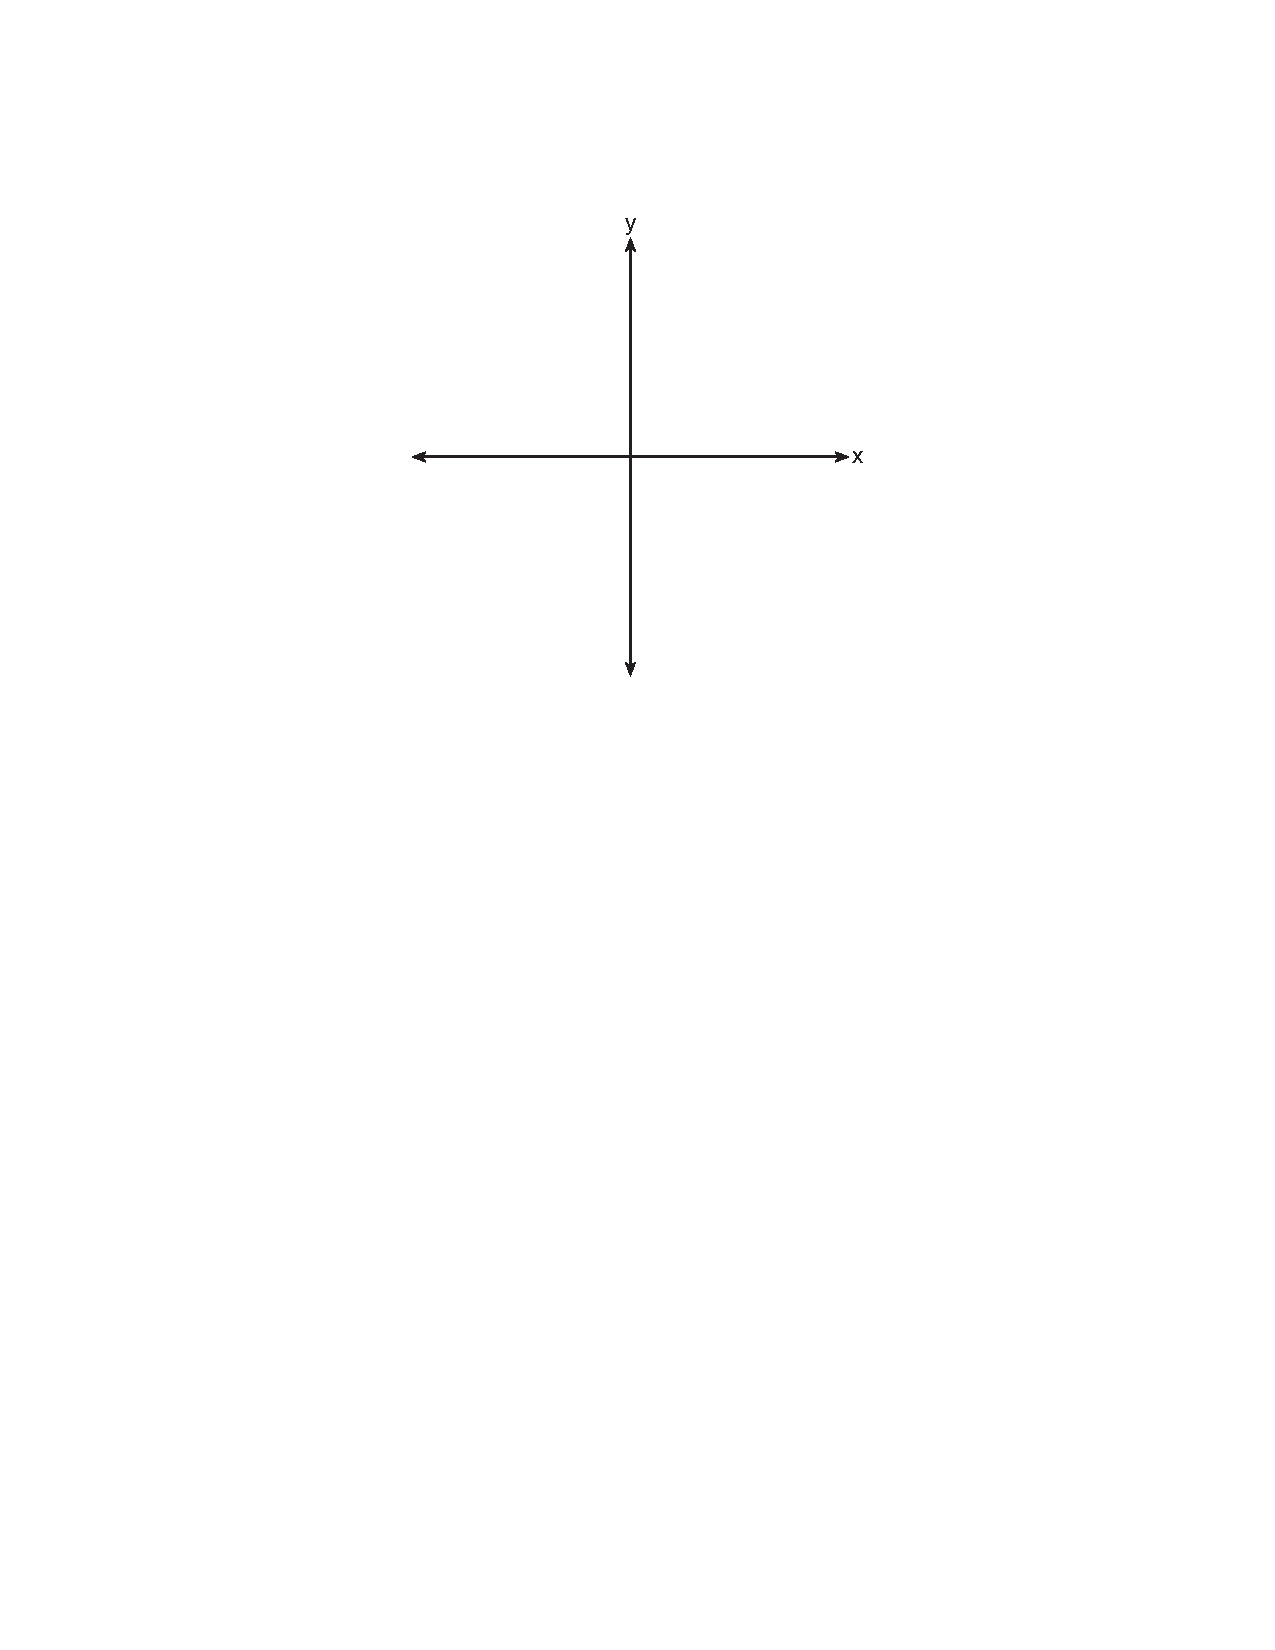
\includegraphics[width=0.65\textwidth]{simple-axes.pdf}
\end{figure}

\newpage
\subsection*{Graphing quadratics}
\item Graph the function $f(x)=-x^2-4x+5$. You may use a graphing calculator rather than factoring the function and completing the square.\\*[5pt]
Label the scales with at least a few values. Mark the vertex as an ordered pair and label each intercept with its value.\\*[20pt]

\begin{figure}[!ht]
    \centering
    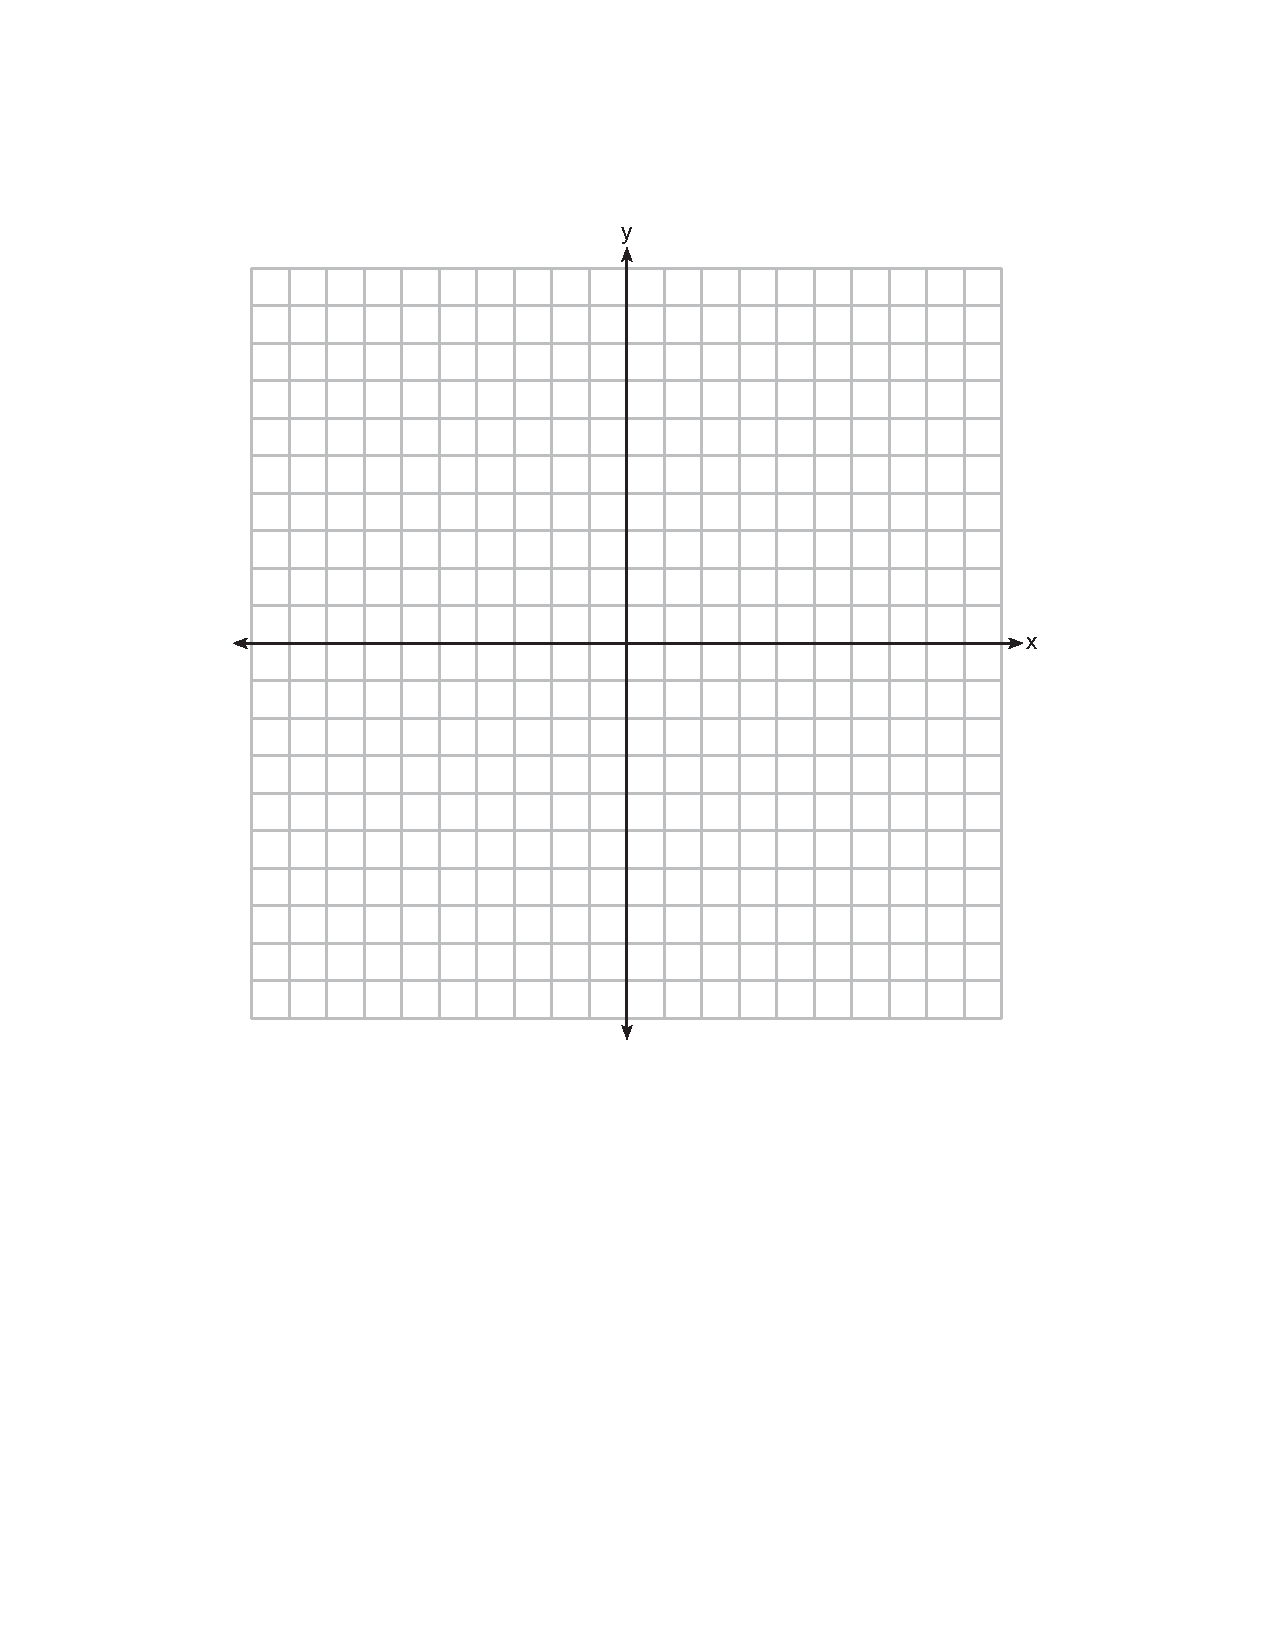
\includegraphics[width=0.75\textwidth]{regents-grid.pdf}
\end{figure}

\newpage
\subsection*{Model situations with quadratic functions}

Use a graphing calculator to view the graph and a table of values for the following function:
\[h(x)=-\frac{1}{225}x^2+\frac{2}{3}x\]
where $h(x)$ represents the height of an object and $x$ it's horizontal position.\\*[5pt]
Make a table of values to the left of the graph, below. Include key values. Graph the function over domain where $h(x) \geq 0$. Use a horizontal scale of 1 square equals 10 units and vertical scale of 1 square equals 2.5 units. Label the intercepts and vertex.\\*[30pt]

\begin{figure}[!ht]
    \flushright
    
\includegraphics[width=0.65\textwidth]{1stQ-grid.pdf}
\end{figure}




\end{enumerate}
\end{document}